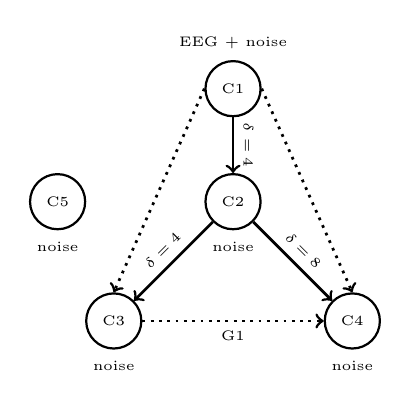
\begin{tikzpicture}[
	font=\tiny,
	every node/.style={transform shape},
	every path/.style={line width=1 pt},
	roundnode/.style={circle, draw=black, thick, minimum size=7mm},
	]
	%Nodes
	\node[roundnode] (c1) {C1};
	\node[above=0.1mm of c1] {EEG + noise};
    % \node[roundnode] (c2) [below=of c1]{C2};	
    \usetikzlibrary{positioning} % for 'below=of'
    \pgfmathsetmacro{\rsqrt}{1/sqrt(2)} % ≈ 0.70710678
    \node[roundnode] (c2) [below=\rsqrt cm of c1]{C2};


    \node[below=0.1mm of c2] {noise};
	\node[roundnode] (c3) [below left=of c2] {C3};
	\node[below=0.1mm of c3] {noise};
	\node[roundnode] (c4) [below right=of c2] {C4};
	\node[below=0.1mm of c4] {noise};
	\node[roundnode] (c5) [left=15mm of c2] {C5};
	\node[below=0.1mm of c5] {noise};
	
	
	%Lines
	\draw[->] (c1.south) -- (c2.north) node[midway, sloped, above] {$\delta = 4$};
	\draw[->] (c2.south west) -- (c3.north east) node[midway, sloped, above] {$\delta = 4$};
	\draw[->] (c2.south east) -- (c4.north west) node[midway, sloped, above] {$\delta = 8$};
	
	\draw[->, dotted] (c1.west) -- (c3.north);
	\draw[->, dotted] (c1.east) -- (c4.north);
	\draw[->, dotted] (c3.east) -- (c4.west) node[midway, sloped, below] {G1};;
	
\end{tikzpicture}